\chapter{Trabalhos Relacionados}
\label{chap2}

\section{Lorem Ipsum}

Lorem ipsum dolor sit amet, consectetur adipiscing elit. Nunc et rutrum tortor. Aenean placerat sed erat at posuere. Praesent a dui augue. Etiam ultrices est in eleifend convallis. Nulla condimentum eleifend nunc, quis commodo nisi imperdiet a. Vestibulum dolor neque, rutrum ac cursus vitae, facilisis et felis. Nam magna massa, molestie ut luctus et, blandit et odio. Vestibulum dignissim, magna quis ultrices convallis, felis sem tempus orci, nec lacinia nibh massa a nulla. Suspendisse potenti. Fusce bibendum tortor quis quam scelerisque sollicitudin. Ut a tempor orci, vel efficitur ante.

\begin{figure}[H]
  \centering
  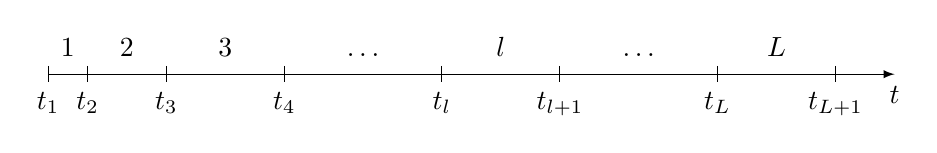
\begin{tikzpicture}
    % draw horizontal line   
    \draw (0,0) -- (0.5,0);
    \draw (0.5,0) -- (1.5,0);
    \draw (1.5,0) -- (3,0);
    \draw (3,0) -- (5,0);
    \draw (5,0) -- (6.5,0);
    \draw (6.5,0) -- (8.5,0);
    \draw (8.5,0) -- (10,0);



    % draw vertical lines
    \foreach \x in {0,0.5,1.5,3,5,6.5,8.5,10}
      \draw (\x cm,3pt) -- (\x cm,-3pt);
      
    \draw[-latex] (10,0) -- (10.75,0) node[below=1pt] {$ t $};      

    % draw nodes
    \draw (0,0) node[below=3pt] {$ t_1 $};
    \draw (0.25,0) node[above=3pt] {$ 1 $};
    \draw (0.5,0) node[below=3pt] {$ t_2 $};
    \draw (1,0) node[above=3pt] {$ 2 $};
    \draw (1.5,0) node[below=3pt] {$ t_3 $}; 
    \draw (2.25,0) node[above=3pt] {$ 3 $};
    \draw (3,0) node[below=3pt] {$ t_4 $};
    \draw (4,0) node[above=3pt] {$ \ldots $};
    \draw (5,0) node[below=3pt] {$ t_l $};
    \draw (5.75,0) node[above=3pt] {$ l $};
    \draw (6.5,0) node[below=3pt] {$ t_{l+1} $};
    \draw (7.5,0) node[above=3pt] {$ \ldots $};
    \draw (8.5,0) node[below=3pt] {$ t_L $};
    \draw (9.25,0) node[above=3pt] {$ L $};
    \draw (10,0) node[below=3pt] {$ t_{L+1} $};
    \draw (10.75,0);
  \end{tikzpicture}
  \label{chap2:timeline}
  %\vspace{-1cm}
  \caption{Intervalos de queima.}  
  \end{figure}

Lorem ipsum dolor sit amet, consectetur adipiscing elit. Nunc et rutrum tortor. Aenean placerat sed erat at posuere. Praesent a dui augue. Etiam ultrices est in eleifend convallis.

\begin{equation}
    \phi_g(\vec{r},t) \cong \phi_g(\vec{r},t_l) \quad \text{para} \quad t \in [t_l,t_{l+1}).
\end{equation}

Aenean purus arcu, auctor sed interdum vel, feugiat a lacus. Fusce nec nibh quis ipsum maximus finibus in at nulla. In non ultricies felis, ac interdum mi Equação \ref{chap2:iso:1}: 

\begin{equation}
    \frac{d}{dt}\underline{N}^n(t) = E_l^n \underline{N}^n(t_l) \quad \text{para} \quad t_l \leq t \leq t_{l+1} \quad l =1,\ldots,L,
    \label{chap2:iso:1}
\end{equation}

\noindent{}com 

\begin{equation*}
    \underline{N}^n(t) \equiv 
    \begin{bmatrix}
    N_1^n(t) \\
    N_2^n(t) \\
    \vdots \\
    N_i^n(t) \\
    \vdots \\
    N_I^n(t)
    \end{bmatrix}.
\end{equation*}